\documentclass[addpoints]{exam}
\usepackage{comment}            
% \begin{comment}                 
% This commented-out block of code translates default words to Spanish. 
% Remove \begin{comment} and \end{comment} to enable it.
\usepackage[spanish]{babel}
\pointpoints{punto}{puntos}
\bonuspointpoints{punto extra}{puntos extra}
\totalformat{Pregunta \thequestion: \totalpoints{} puntos}
\chqword{Pregunta}
\chpgword{Página}
\chpword{Puntos}
\chbpword{Puntos extra}
\chsword{Puntos obtenidos}
\chtword{Total}
% \end{comment}
\usepackage{datetime}
\usepackage{graphicx}
\usepackage{tabularx}
\usepackage{booktabs}
\boxedpoints
\newdate{testdate}{27}{05}{2025}

 \pagestyle{headandfoot}
 \runningheadrule
 \firstpageheader{\displaydate{testdate}}{\textbf{Escuela Politécnica Nacional}\\\textbf{Arquitectura de Computadores ICCD332}\\Prueba}{\textbf{Prof:} Lenin G. Falconí}
 \runningheader{ICCD332}
 {Prueba, Página \thepage\ de \numpages}
 {\displaydate{testdate}}
 \firstpagefooter{}{}{}
 \runningfooter{}{}{}

 \begin{document}
% Quito, \displaydate{testdate} \hfill \textbf{Profesor:} Lenin
% G. Falconí M.Sc.                %
% -------------------------------------------------------------
% This code creates the text before the first question
% -------------------------------------------------------------
\begin{center}
  \fbox{\fbox{\parbox{5.5in}{ Conteste las siguientes preguntas en su
        hoja de respuestas. Este es un examen de procedimientos por lo
        que puede usar calculadora para realizar operaciones. Todos
        los procedimientos deben quedar detallados.Los resultados
        deben quedar marcados con esferográfico. Al terminar el
        examen,tome capturas fotográficas del mismo y suba al aula
        virtual.}}}
\end{center}

\vspace{5mm}

\vspace{5mm}
\makebox[\textwidth]{Nombres Completos:\enspace\hrulefill}
\vspace{5mm}

% \makebox[\textwidth]{Instructor’s name:\enspace\hrulefill}


% -------------------------------------------------------------

%Here, the questions begin
\begin{questions}

%First question below
  % \question[1 \half] Complete la siguiente tabla con las representaciones de
  % números enteros con signo solicitadas. Exprese sus resultados en
  % binario usando 8 bits.


  % \begin{tabularx}{\textwidth}{|X|X|X|X|X|}
  %   \hline
  %   \textbf{Número} & \textbf{Comp a 1} & \textbf{Comp a 2} & \textbf{Signo Magnitud} & \textbf{Número Base 10} \\
  %   \hline
  %   $-173_{8}$ &  &  &  & \\
  %   \hline
  %   $+7B_{16}$ &  &  &  & \\
  %   \hline
  %   $-30_{16}$ &  &  &  & \\
  %   \hline
  % \end{tabularx}

 
\question Dado $-173_8$, en una arquitectura de 8 bits, obtenga las
  representaciones solicitadas en hexadecimal
%This question has several parts
\begin{parts}
\part[\half] Representación en complemento a 1
%\vspace*{\stretch{2}} %Equally distributes the available space

\part[\half] Representación en complemento a 2
%\vspace*{\stretch{2}}
\part[\half] Representación en signo magnitud.
%\vspace*{\stretch{2}}
\end{parts}

\droptotalpoints %Prints the number of points in this question

%The next two questions are multiple choice examples
% -------------------------------------------------------------
% \question Which of these famous physicists invented time?

% \begin{oneparchoices}
%  \choice Stephen Hawking 
%  \choice Albert Einstein
%  \choice Emmy Noether
%  \choice This makes no sense
% \end{oneparchoices}

% \question Which of these famous physicists published a paper on Brownian Motion?

% \begin{checkboxes}
%  \choice Stephen Hawking 
%  \choice Albert Einstein
%  \choice Emmy Noether
  
%  \choice I don't know
% \end{checkboxes}
% -------------------------------------------------------------

\question Obtenga el complemento $r^n-X$ cuando $r=16$ y
  $X=CB_{16}$. Considere una arquitectura de 8 bits. Exprese el
  resultado en hexadecimal y binario.

% \begin{itemize}

  
% \item $56_{10}-63_{8}$

% \end{itemize}
\begin{parts}
  \part[\half] Obtener el complemento en la base
 % \vspace*{\stretch{2}}

  \part[\half] ¿Cuál es el número original en representación entera
    con signo en decimal?
 %  \vspace*{\stretch{2}}

\end{parts}
\droptotalpoints %Prints the number of points in this question

\question[1 \half] Dado el número $X=228_8$, obtenga el complemento a 2 de
  $\frac{X}{2}$. Escriba el resultado en hexadecimal.

%\vspace*{\stretch{2}}

% \question Simplifique la siguiente expresión
% $F=\bar{A}C+\bar{A}B+A\bar{B}C+BC$
% \begin{parts}
%   \part[\half] Usando postulados del álgebra de Boole
% %  \vspace*{\stretch{2}}
%   \part[\half] Usando Mapa K
% %  \vspace*{\stretch{2}}
% \end{parts}
\droptotalpoints

% \question El complemento en la base de un número $A$ en base $r$ se
% define como $r^n-A$. Obtenga:

% \begin{parts}
%   \part[\half] Complemento a 16 de AF3B
%   \vspace*{\stretch{2}}
%   \part[\half] Convierta AF3B a binario y obtenga el complemento a 2
%   \vspace*{\stretch{2}}
%   \part[\half] Convierta el resultado anterior a hexadecimal
% \end{parts}
% \droptotalpoints %Prints the number of points in this question

%\clearpage

% \makebox[\textwidth]{Nombres Completos:\enspace\hrulefill}
% \vspace*{\stretch{2}}
\question[2] Exprese en formato IEEE de 32 bits el número
$-32.25$. Escriba el resultado en notación hexadecimal. %\answerline
\droptotalpoints


\question[2] Obtenga el valor decimal equivalente del número expresado en
formato  IEEE de 32 bits: $0x70E50000$. Utilice una precisión de 7
dígitos decimales en su respuesta%\answerline
%\vspace*{\stretch{2}}
\droptotalpoints

\question En una arquitectura de 8 bits, $A^{SM}=0xE4$ y
  $B^{SM}=0x7D$ son números en representación signo magnitud. Exprese
  los siguientes resultados en hexadecimal.
\begin{parts}
  \part[1] Obtener la suma en complemento a 2 de sus valores
    absolutos i.e. $|A^{SM}|+|B^{SM}|$
%  \vspace*{\stretch{2}}
  \part[1] Obtener la diferencia $|A^{SM}|-|B^{SM}|$ en complemento a 2 de sus valores
    absolutos. 
%  \vspace*{\stretch{2}}
\end{parts}
\droptotalpoints
% \question[2] Se desea diseñar un circuit para alarma de un automóvil
% que consta de 3 sensores:
% \begin{itemize}
% \item Interruptor de encendido del coche $I$
% \item Sensor de la puerta del coche $S_P$
% \item Sensor de luces frontales $S_L$
% \end{itemize}
% Obtenga la tabla de verdad y simplifique usando Mapas K para obtener
% el circuito en compuertas NAND que active la alarma en las siguientes
% condiciones:

% \begin{itemize}
% \item Las luces frontales están prendidas $S_L=1$, mientras el
%   interruptor del encendido está apagado $I = 0$.
% \item La puerta está abierta $S_p=0$ mientras el interruptor de
%   encendido está activado $I=1$
% \end{itemize}

% Realice la tabla y el mapa en el orden de variables $I$, $S_P$, $S_L$
% \begin{figure}[h!]
%   \centering
%   \caption{Circuito de Alarma de Vehículo}
%   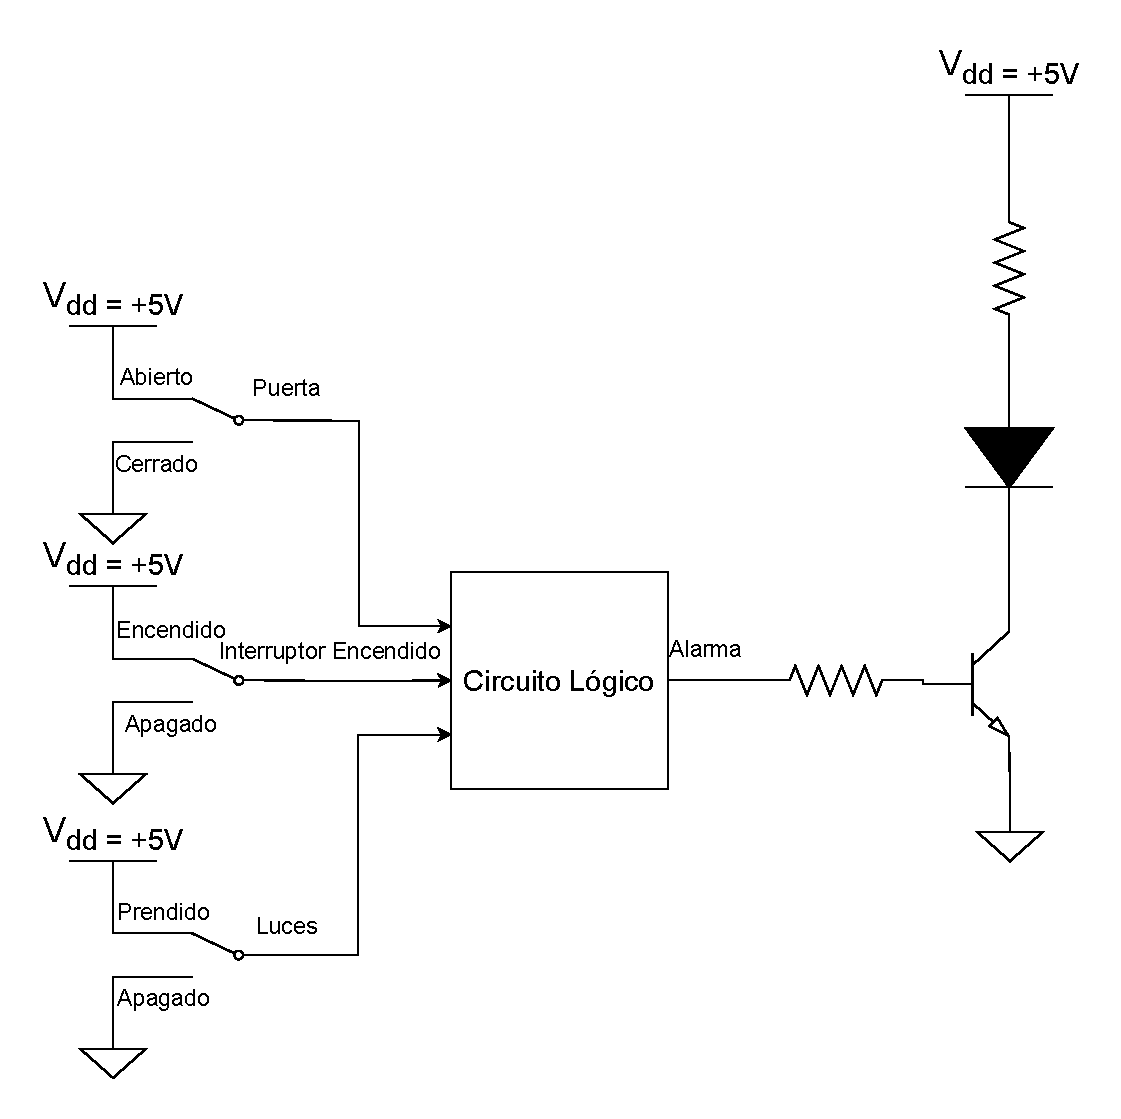
\includegraphics[scale=0.6]{./images/Problema4-8.pdf}
%   \label{fig:circuito}
% \end{figure}


\end{questions}

\begin{center}
  \scriptsize
  \combinedgradetable[h][questions]
\end{center}

\end{document}

%%% Local Variables:
%%% mode: LaTeX
%%% TeX-master: t
%%% End:
